%-------------------------------------------------------------------------------------------------------
%                                                            HEADER
%-------------------------------------------------------------------------------------------------------
% ¿Qué secciones debe contener una presentación?

% Índice
% Introducción al tema
% Desarrollo del proyecto
% Conclusiones 
% Trabajo Futuro
% Invitación a preguntas
% Agradecimiento y despedida
 
% ¿Aproximadamente cuántas filminas?

% Lo ideal es que la presentación ronde los 30min (y no exceda los 40min). Si en promedio dedicamos 3min por filmina, 10 a 12 filminas útiles es un número razonable. Con "útiles" me refiero a las de contenido, no separadores ni indicativas.

% Recuerden que lo importante es lo que uds. hicieron. El marco teórico está en el informe y con 1 o 2 filminas debería ser suficiente.

% INSERTAR FIGURAS EJEMPLO
%\begin{figure}[ht]
%    \centering
%    \vspace{-0.50cm}
%    \scalebox{0.25}{\includegraphics[angle=0]{./oh_source.eps}}
%\end{figure}

\documentclass{beamer}
\graphicspath{{./figuras/}}
\mode<presentation>
{
    \usebackgroundtemplate{
\includegraphics[width=\paperwidth]{fondo_2.jpg}}
    \usetheme{default}      % or try Darmstadt, Madrid, Warsaw, default...
    \usecolortheme{default} % or try albatross, beaver, crane, default ...
    \usefonttheme{default}  % or try serif, structurebold, ...
    \setbeamertemplate{navigation symbols}{}
    \setbeamertemplate{caption}[numbered]
} 

\usepackage[english]{babel}
\usepackage[utf8x]{inputenc}

\title[Your Short Title]{Infraestructura tecnológica virtual con automatización y orquestación.}
\author{Arese, Juan Pablo - Diers, Werner Christian}
\institute{Facultad de Ciencias Exactas, Físicas y Naturales - UNC}
\date{Marzo 2017}

\begin{document}


%-------------------------------------------------------------------------------------------------------
%                                                                TITULO
%-------------------------------------------------------------------------------------------------------
\begin{frame}
  \titlepage
\end{frame}


%-------------------------------------------------------------------------------------------------------
%                                                   ORGANIZACIÓN DE LA PRESENTACIÓN
%-------------------------------------------------------------------------------------------------------
\section{Organización de la Presentación}

\begin{frame}{Organización de la Presentación}
    \vspace{-1cm}
    \begin{itemize}
        \item Introducción
        \item Objetivos
        \item Arquitectura
        \item Desarrollo del sistema
        \begin{itemize}
            \item Servidor web
            \item Servidor de virtualización
            \item Servidor de aprovisionamiento
            \item Servidor de orquestación          
        \end{itemize}
        \item Conclusión
        \begin{itemize}
            \item Trabajos futuros
        \end{itemize}
        \item Demostración
    \end{itemize}

\end{frame}


%-------------------------------------------------------------------------------------------------------
%                                                             INTRODUCCION
%-------------------------------------------------------------------------------------------------------
\section{Introducción}

\begin{frame}
    %\vspace{}
    \Huge
    \centering
    \textbf{Introducción}

\end{frame}


\begin{frame}{Introducción}
    \vspace{0cm}
    Una infraestructura moderna implica:
    \begin{itemize}
        \item Costos
        \item Rendimiento computacional
        \item Aplicación de políticas
                \begin{itemize}
                    \item Configuraciones establecidas por cada entidad
                    \item Estandarización de los recursos y parámetros utilizados
        \end{itemize}
        \item Agilidad
    \end{itemize}
\end{frame}

\begin{frame}{Introducción}
    \vspace{0cm}
    \textbf{¿Qué es virtualización?}
    \begin{block}{}
        \textbf{Software ejecutándose}, de forma \textbf{concurrente} y \textbf{aislada de otros procesos} en el mismo sistema.
    \end{block}
    \begin{block}{}
        Es la manera más eficaz de \textbf{reducir los costos} y \textbf{aumentar la  agilidad} de cualquier organización.
    \end{block}
    % \begin{itemize}
    %     \item Software ejecutándose
    %     \item Concurrencia
    %     \item Aislamiento
    %     %\item Hypervisor
    % \end{itemize}
    % Virtualización es un término para software ejecutándose, usualmente sistemas operativos, de manera concurrente y aislada de otros programas en el mismo sistema. 

    % \begin{block}{}
    %     Muchas de las implementaciones de virtualización utilizan un hypervisor, una capa de software que controla el hardware y provee sistemas operativos huéspedes con acceso a los dispositivos de hardware subyacentes. 
    % \end{block}

    % \begin{block}{}
    %     El hypervisor permite ejecutar múltiples sistemas operativos en el mismo sistema físico ofreciendo hardware virtualizado al sistema operativo huésped.
    % \end{block}

\end{frame}

\begin{frame}{Introducción}
    \vspace{0cm}
    \textbf{¿Qué es aprovisionamiento?}
    \\
    Aprovisionar es proveer o hacer que algo esté disponible. En el \textbf{contexto de esta presentación}, aprovisionar es el \textbf{conjunto de acciones} requeridas para preparar una máquina virtual para su uso básico.

    \begin{itemize}
        \item Disco
        \item Memoria RAM
        \item CPU
        \item Sistema operativo
        \item Servicios
        \item Configuración
    \end{itemize}
    % En general, aprovisionamiento, significa proveer o hacer que algo esté disponible. El término es utilizado en un gran variedad de contextos en el área de Tecnologías de Información. En este Proyecto Integrador, el término hace referencia a lo siguiente:

    % \begin{block}{}
    % \textit
    % {
    %     Aprovisionamiento es el conjunto de acciones para preparar una máquina virtual, con el sistema apropiado, datos y software dejándola lista para su operación.
    % }
    % \end{block}

\end{frame}

\begin{frame}{Introducción}
    \vspace{0cm}
    \textbf{¿Qué es orquestación?}
    \begin{itemize}
        \item Automatizar procesos y flujos de trabajo.
        \item Consistencia de la infraestructura.
        \item Infraestructura como código.
        \item Integrar servicios rápidamente.
    \end{itemize}
    % Orquestación es automatizar procesos y flujos de trabajo, mientras que la automatización básicamente automatiza una tarea específica.
    % Un orquestador es una pieza de software que permite integrar servicios provenientes de diversas fuentes, y proveer información de forma síncrona o asíncrona, a través del uso de servicios web, bases de datos, archivos, entre otras fuentes y destinos.

\end{frame}
%-------------------------------------------------------------------------------------------------------
%                                                           OBJETIVOS
%-------------------------------------------------------------------------------------------------------
\section{Objetivos}

\begin{frame}
    %\vspace{}
    \Huge
    \centering
    \textbf{Objetivos}

\end{frame}

\begin{frame}{Objetivos}
    \vspace{0cm}
    Integrar diferentes herramientas con el fin de implementar técnicas de \textbf{orquestación}, virtualización, instalación y \textbf{configuración automática} para facilitar la \textbf{gestión de servidores} virtuales y sus servicios asociados.

\end{frame}

%
%\begin{frame}{Objetivos secundarios}
%\vspace{0cm}
%\begin{itemize}
%    \item Instalar y utilizar sistemas operativos para servidor
%    \item Emplear herramientas de virtualización
%    \item Usar herramientas de aprovisionamiento
%    \item Utilizar herramientas de orquestación
%    \item Analizar protocolos para booteo a través de la red
%\end{itemize}
%
%\end{frame}


%-------------------------------------------------------------------------------------------------------
%                                                            ARQUITECTURA
%-------------------------------------------------------------------------------------------------------
\section{Arquitectura}

\begin{frame}
    %\vspace{}
    \Huge
    \centering
    \textbf{Arquitectura}

\end{frame}

\begin{frame}{Arquitectura}
    \vspace{0cm}
    La arquitectura implementada es la de cliente - servidor. 
    \vspace{0.5cm}
    \\
    En esta arquitectura, múltiples clientes \textbf{realizan peticiones} a los servidores, los cuales les \textbf{dan respuesta}.
    \vspace{0.5cm}
    \\
    El sistema cuenta con 4 servidores principales, un servidor de máquinas virtuales, uno de aprovisionamiento, otro de orquestación y un servidor web. 
    %\begin{itemize}
    %    \item Crear las máquinas virtuales
    %    \item Asignar direcciones IP por medio del protocolo DHCP
    %    \item Proveer a la máquina con el sistema operativo deseado y los parámetros de configuración establecidos
    %    \item Orquestar las políticas definidas para una máquina o un conjunto de máquinas
    %\end{itemize}

\end{frame}

\begin{frame}{Arquitectura}
    \vspace{0.5cm}
    \begin{figure}[ht]
       \centering
       \vspace{-0.50cm}
       \scalebox{0.35}{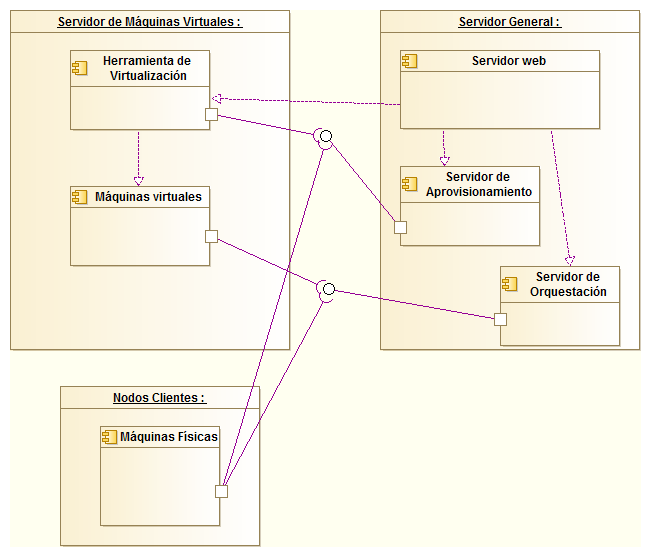
\includegraphics[angle=0]{./figuras/arquitectura.png}}
    \end{figure}

\end{frame}

\begin{frame}{Arquitectura}
    \vspace{0.5cm}
    \begin{figure}[ht]
       \centering
       \vspace{-0.50cm}
       \scalebox{0.3}{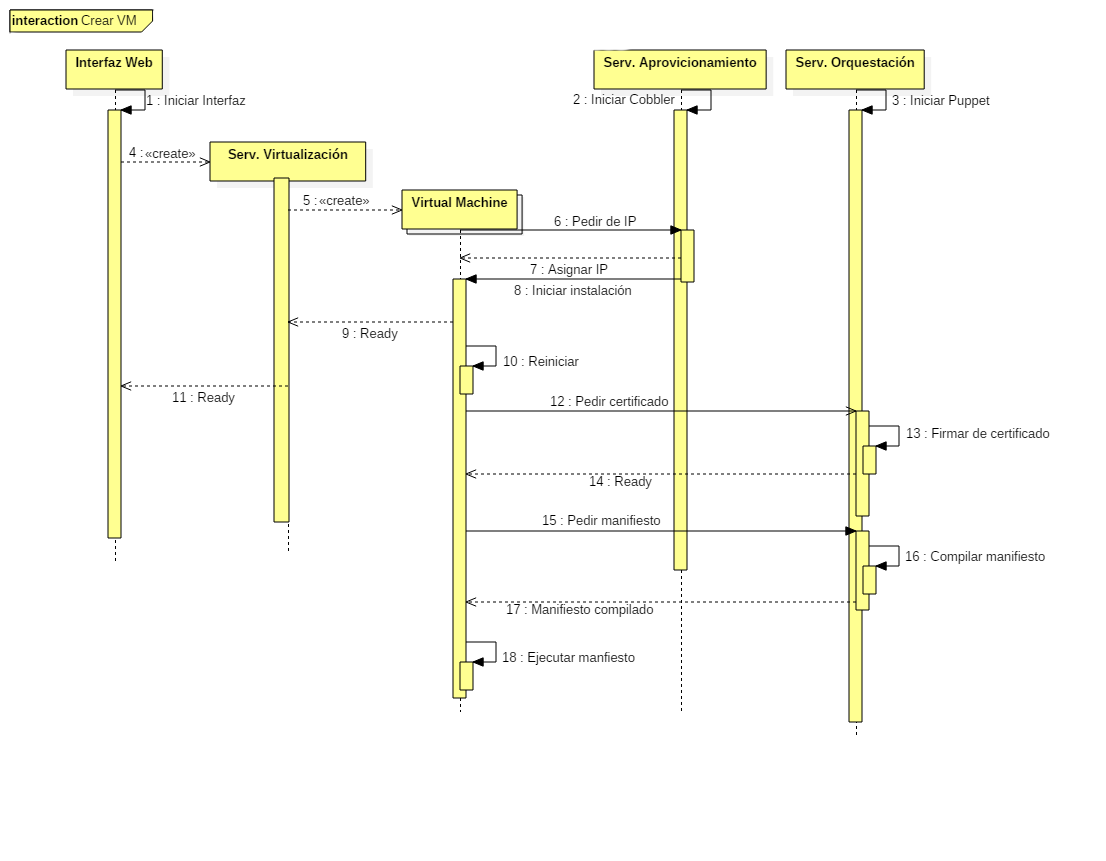
\includegraphics[angle=0]{./figuras/Crear_VM.png}}
    \end{figure}

\end{frame}



%-------------------------------------------------------------------------------------------------------
%                                                                DESARROLLO
%-------------------------------------------------------------------------------------------------------
\section{Desarrollo}
\begin{frame}
    %\vspace{}
    \Huge
    \centering
    \textbf{Desarrollo}

\end{frame}

% -  -  -  -  -  -  -  -  -  -  -  -  -  -
%           INTERFAZ WEB
% -  -  -  -  -  -  -  -  -  -  -  -  -  -

\begin{frame}
    %\vspace{}
    \Huge
    \centering
    \textbf{Servidor Web}

\end{frame}

\begin{frame}{Desarrollo - Servidor Web}
    \vspace{0cm}
    Se utilizó la herramienta Python Bottle para la realización del servidor web, dado que es un WSGI (Web Server Gateway Interface) rápido, sencillo y ligero.
    \\
    \vspace{0.5cm}
    Los \textbf{GET} y \textbf{POST} son \textit{decorators} que enlazan una pieza de código con una URL. 
    %La herramienta utilizada para crear la interfaz web fue Python Bottle.
    %\begin{itemize}
    %    \item Es un WSGI (Web Server Gateway Interface) rápido, sencillo y ligero
    %    \item Distribuído como un módulo único
    %    \item Su única dependencia es la Librería Estándar de Python
    %    \item Puede ejecutarse como un servidor web autónomo
    %    \item Plugins para bases de datos populares
    %\end{itemize}
    
\end{frame}

\begin{frame}{Desarrollo - Servidor Web}
    \vspace{0cm}
    \begin{figure}[ht]
       \centering
       \scalebox{0.4}{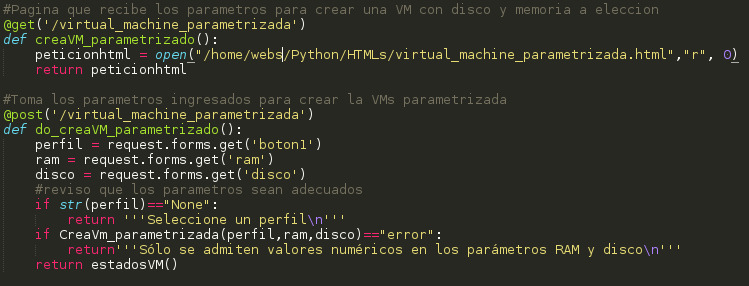
\includegraphics[angle=0]{./figuras/get-post.png}}
    \end{figure}
    \begin{figure}[ht]
       \centering
       \scalebox{0.4}{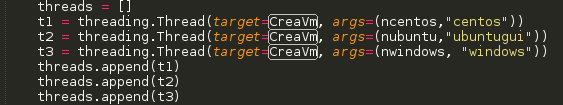
\includegraphics[angle=0]{./figuras/Hilos.png}}
    \end{figure}

\end{frame}

\begin{frame}{Desarrollo - Servidor Web}
    \vspace{0cm}
    \begin{figure}[ht]
       \centering
       \scalebox{0.3}{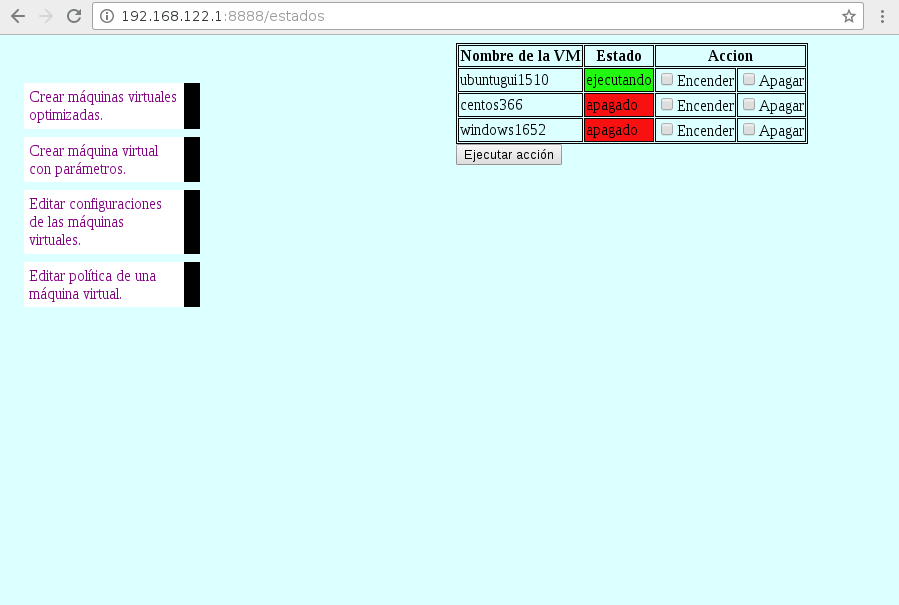
\includegraphics[angle=0]{./figuras/interfaz_web_4.png}}
    \end{figure}

\end{frame}

% -  -  -  -  -  -  -  -  -  -  -  -  -  -
%           VIRTUALIZACION
% -  -  -  -  -  -  -  -  -  -  -  -  -  -

\begin{frame}
    %\vspace{}
    \Huge
    \centering
    \textbf{Virtualización}

\end{frame}


\begin{frame}{Desarrollo - Servidor de virtualización}
    \vspace{0cm}
    Existen diferentes tipos de virtualización. Nosotros aplicamos \textbf{virtualización completa}. 
    \\
    La herramienta utilizada fue KVM/Qemu.
    \begin{itemize}
        \item El sistema operativo huésped \textbf{desconoce} que está en un entorno virtual
        \item El hardware se encuentra virtualizado por el sistema operativo anfitrión
        \item La capa de virtualización, el \textbf{hypervisor}, media entre los sistemas huéspedes y el anfitrión
    \end{itemize}

\end{frame}

\begin{frame}{Desarrollo - Servidor de virtualización}
    \vspace{0cm} {Esquema de virtualización completa}
    \vspace{0.5cm}
    \begin{figure}[ht]
       \centering
       \vspace{-0.50cm}
       \scalebox{0.60}{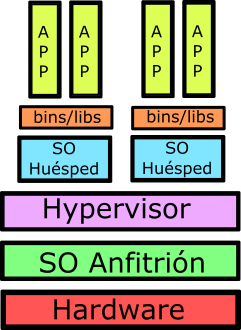
\includegraphics[angle=0]{./figuras/virtualizacion_tipos_3.png}}
    \end{figure}

\end{frame}

\begin{frame}{Desarrollo - Servidor de virtualización}
    \vspace{0cm} {Arquitectura de KVM}
    \vspace{0.5cm}
    \begin{figure}[ht]
       %\centering
       \raggedright
       \vspace{-0.50cm} 
       \scalebox{0.25}{\hspace*{8cm}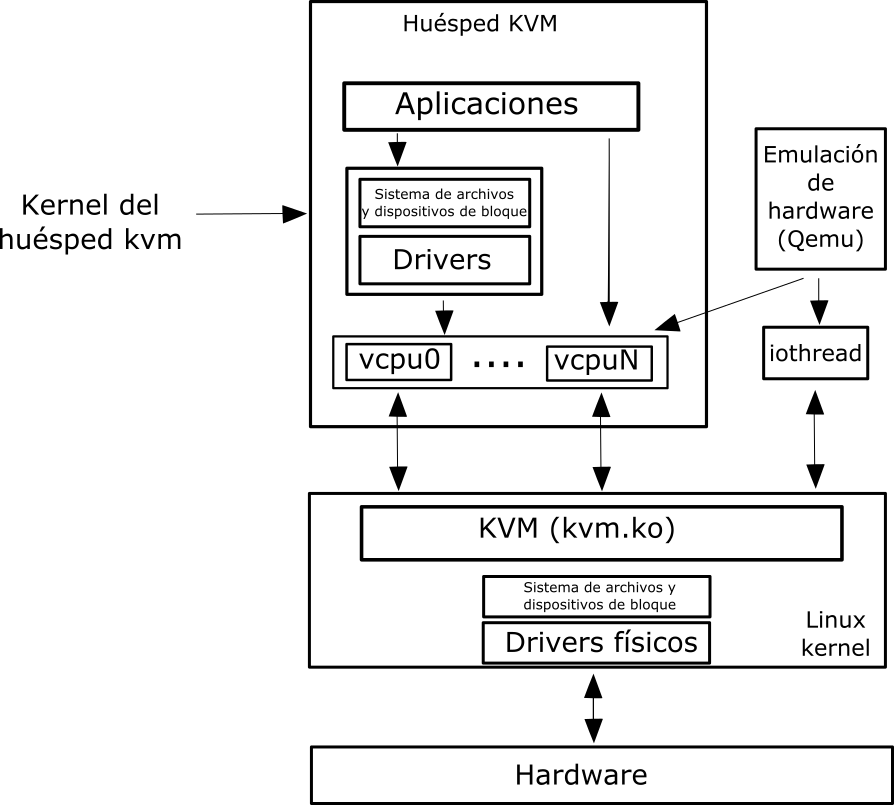
\includegraphics[angle=0]{./figuras/kvm_arquitectura_1.png}}
    \end{figure}

\end{frame}

\begin{frame}{Desarrollo - Servidor de virtualización}
    \vspace{-1cm} {Ejemplo de creación de una máquina virtual}
    \\
    \vspace{0.5cm}
    \begingroup
    \fontsize{8pt}{12pt}\selectfont
        \texttt{
        \# virt-install \textbackslash \\
           \hspace{0.75cm} --connect qemu:///system \textbackslash \\
           \hspace{0.75cm} --name=nodo-01 \textbackslash \\
           \hspace{0.75cm} --disk path=/var/lib/libvirt/images/centos-vm.qcow2,size=25 \textbackslash \\
           \hspace{0.75cm} --graphics spice \textbackslash \\
           \hspace{0.75cm} --vcpus=2 --ram=3072 \textbackslash \\
           \hspace{0.75cm} --network network=puppet, mac="52:54:00:d5:a1:76" --pxe \textbackslash \\
           \hspace{0.75cm} --os-type=linux \textbackslash \\
           \hspace{0.75cm} --os-variant=centos7 \textbackslash \\
           \hspace{0.75cm} --description "nodo con CentOS 7" \textbackslash  \\
           \hspace{0.75cm} --arch=x86-64 \textbackslash \\
           \hspace{0.75cm} --accelerate \textbackslash \\
        }    
    \endgroup    
\end{frame}

\begin{frame}{Desarrollo - Servidor de virtualización}
    \vspace{-1cm} {Obtener información acerca de un máquina virtual}
    \\
    \vspace{0.5cm}
    \begingroup
    \fontsize{8pt}{8pt}\selectfont
        \texttt{
            \# virsh list --all \\
             Id\hspace{0.15cm}  Name\hspace{1.5cm} State \\
            ---------------------------- \\
             1\hspace{0.15cm}   ubuntu-1720\hspace{0.5cm}   stopped \\
             2\hspace{0.15cm}   centos-1575\hspace{0.5cm}   stopped \\
             3\hspace{0.15cm}   centos-1575\hspace{0.5cm}   running \\
             4\hspace{0.15cm}   ubuntu-2285\hspace{0.5cm}   running \\
             5\hspace{0.15cm}   windows-7295\hspace{0.38cm}  stopped \\
            \vspace{0.5cm}
             \# virsh dominfo  centos-1516  \\
             id:\quad 3 \\
             name:\quad centos-1516  \\
             uuid:\quad  4a4c59a7-ee3f-c781-96e4-288f2862f011 \\
             os type:\quad linux \\
             state:\quad running  \\
             cpu(s):\quad  2  \\
             cpu time:\quad  11.0s \\ 
             max memory:\quad   512000 kb  \\
             used memory:\quad  512000 kb  \\
        }    
    \endgroup    
\end{frame}

% -  -  -  -  -  -  -  -  -  -  -  -  -  -
%           APROVISIONAMIENTO
% -  -  -  -  -  -  -  -  -  -  -  -  -  -

\begin{frame}
    %\vspace{}
    \Huge
    \centering
    \textbf{Aprovisionamiento}

\end{frame}

\begin{frame}{Desarrollo - Servidor de aprovisionamiento}
    \vspace{0cm}
    El centro del servidor de aprovisionamiento es Cobbler. Además de este, encontramos servidores PXE, DHCP, TFTP, SAMBA y DNS.
    \vspace{0.5cm}
    \\ 
    El servidor Cobbler se \textbf{basa en objetos} para definir la instalación y configuración deseada en cada caso.
    \\
    Los objetos se ordenan en una  \textbf{jerarquía vertical}, donde el objeto inferior, contiene a los superiores.
    %La herramienta utilizada para el aprovisionamiento fue Cobbler.
    %\\
    %Utiliza una arquitectura cliente - servidor.
    %\begin{itemize}
    %    \item El servidor debe ejecutarse en un sistema basado en Unix
    %    \item Centraliza y simplifica el control de servicios incluyendo PXE, DHCP, TFTP y DNS con propósito de realizar instalaciones basadas en red de sistemas operativos
    %    \item Cobbler utiliza objetos para definir la configuración de aprovisionamiento:
    %\end{itemize}
    
\end{frame}

\begin{frame}{Desarrollo - Servidor de aprovisionamiento}
    \vspace{0cm} {Modelado de Cobbler}
    \vspace{0.5cm}
    \begin{figure}[ht]
       \centering
       \vspace{-0.50cm}
       \scalebox{0.32}{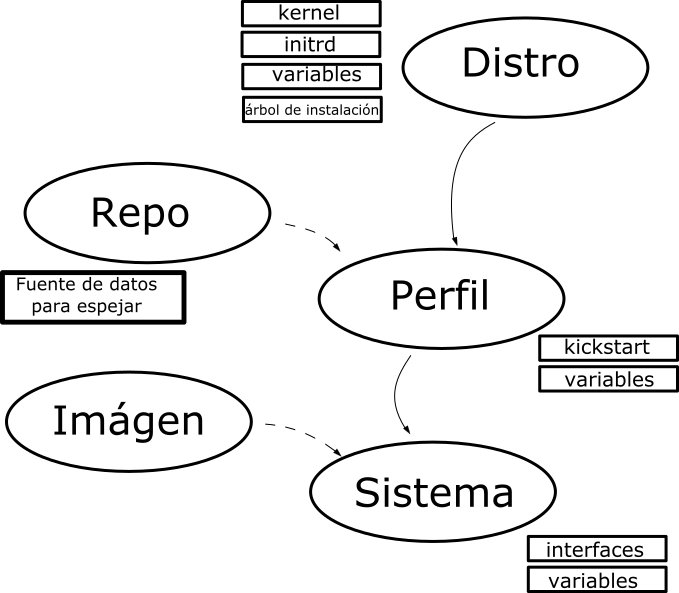
\includegraphics[angle=0]{./figuras/cobbler_modelado.png}}
    \end{figure}
\end{frame}

\begin{frame}{Desarrollo - Servidor de aprovisionamiento}
    \vspace{0cm}
    \begin{itemize}
        \item \textbf{Distro}: Distribución que se desea instalar
        \item \textbf{Repo}: Repositorio, sitio centralizado donde se almacena y mantiene información digital
        \item \textbf{Perfil}: Asocia una distribución a opciones especializadas adicionales, como puede ser un archivo de configuración
        \item \textbf{Imágen}: Copia del estado de un sistema computacional, guardado en un archivo o disco
        \item \textbf{Sistema}: Mapea una pieza de hardware (o una máquina virtual) con el perfil asignado a correr en ella
    \end{itemize}

\end{frame}

\begin{frame}{Desarrollo - Servidor de aprovisionamiento}
    \vspace{0.5cm}
    \begin{figure}[ht]
       \centering
       \vspace{-0.50cm}
       \scalebox{0.55}{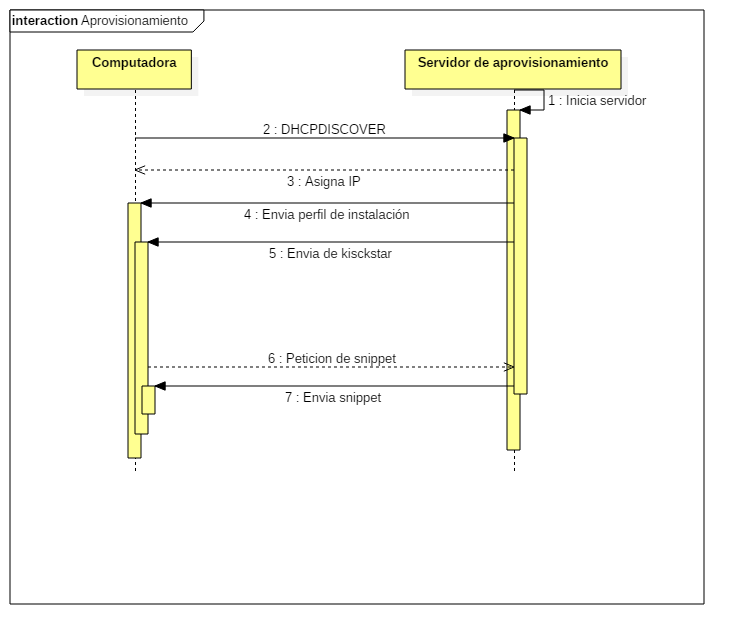
\includegraphics[angle=0]{./figuras/Aprovisionamiento.png}}
    \end{figure}
\end{frame}


%
% -  -  -  -  -  -  -  -  -  -  -  -  -  -
%           ORQUESTACION
% -  -  -  -  -  -  -  -  -  -  -  -  -  -

\begin{frame}
    %\vspace{}
    \Huge
    \centering
    \textbf{Orquestación}

\end{frame}

\begin{frame}{Desarrollo - Servidor de orquestación}
    \vspace{0cm}
    El servidor usado para orquestar fue Puppet. 
    \begin{itemize}
        \item Tiene soporte para la administración de \textbf{múltiples plataformas}.
        \item Los recursos del sistema y sus estados se configuran utilizando un \textbf{lenguaje declarativo propio}.
        \item Estas configuraciones se denominan \textbf{manifiestos}.
        \item Las comunicaciones se realizan bajo \textbf{HTTPS}.

    \end{itemize}

\end{frame}


\begin{frame}{Desarrollo - Servidor de orquestación}
    \vspace{0cm} {Ciclo de orquestación}
    \vspace{0cm}
        \begin{figure}[ht]
           \centering
           \scalebox{0.5}{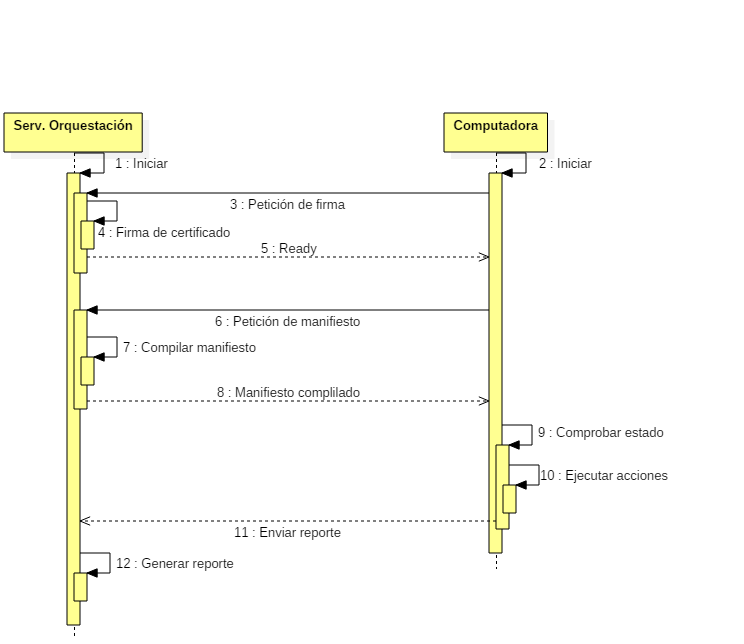
\includegraphics[angle=0]{./figuras/Orquestacion.png}}
        \end{figure}

\end{frame}

%\begin{frame}{Desarrollo - Orquestación}
%    \vspace{0cm} {Nodos administrados}
%    \vspace{0cm}
%    \begin{figure}[ht]
%       \centering
%       \scalebox{0.6}{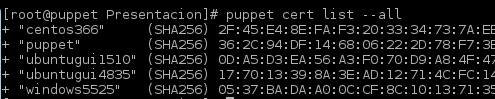
\includegraphics[angle=0]{./figuras/puppet_nodos.png}}
%    \end{figure}
%
%\end{frame}

\begin{frame}{Desarrollo - Servidor de orquestación}
    \vspace{0cm} {Estructura de los módulos de Puppet}
    \vspace{0cm}
    \begin{figure}[ht]
       \centering
       \scalebox{0.4}{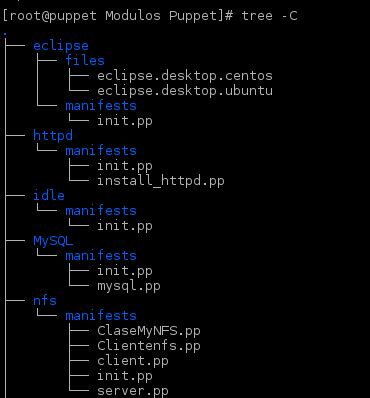
\includegraphics[angle=0]{./figuras/orquestacion-modulos-puppet.png}}
    \end{figure}

\end{frame}

\begin{frame}{Desarrollo - Servidor de orquestación}
    \vspace{0cm} {Ejemplo lenguaje declarativo de Puppet}
    \vspace{0cm}
    \begin{figure}[ht]
       \centering
       \scalebox{0.5}{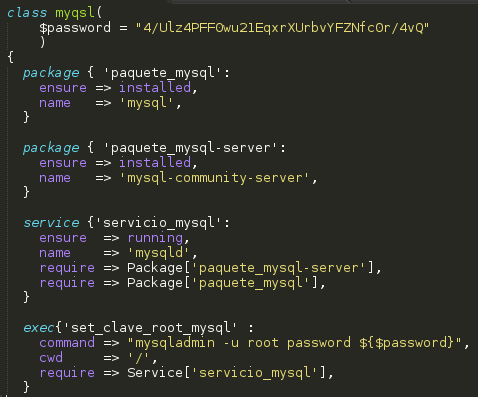
\includegraphics[angle=0]{./figuras/orquestacion-codigo-puppet-1.png}}
    \end{figure}

\end{frame}

\begin{frame}{Desarrollo - Servidor de orquestación}
    \vspace{0cm} {Ejemplo lenguaje declarativo de Puppet}
    \vspace{0cm}
    \begin{figure}[ht]
       \centering
       \scalebox{0.4}{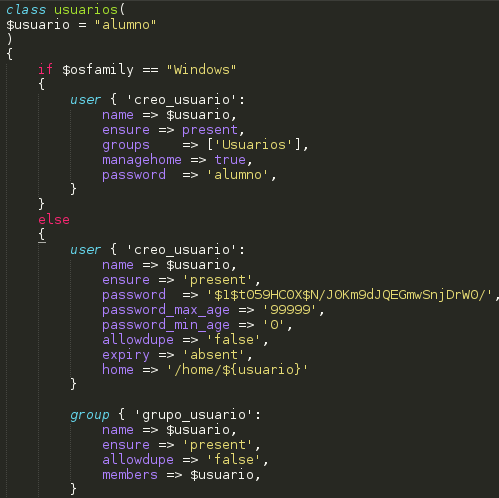
\includegraphics[angle=0]{./figuras/orquestacion-codigo-puppet-2.png}}
    \end{figure}

\end{frame}
%-------------------------------------------------------------------------------------------------------
%                                                               CONCLUSIONES
%-------------------------------------------------------------------------------------------------------
\section{Conclusiones}
\begin{frame}
    %\vspace{}
    \Huge
    \centering
    \textbf{Conclusiones}

\end{frame}

\begin{frame}{Conclusiones}
    \vspace{0cm}

    El sistema obtenido, es un \textbf{sistema modularizado}. Cada tarea es realizada por un servidor de forma independiente al resto. 
    \\
    \vspace{0.5cm}
    Se implementó un diseño que permite \textbf{escalabilidad y mejoras a futuro}.
    \\
    \vspace{0.5cm}  
    Si bien se encontró una solución basada en \textbf{herramientas libres}, estas no siempre permiten situarse en la \textbf{cresta de la ola}.
    %\begin{itemize}
    %    \item Solución modularizada
    %    \item Permite la escalabilidad
    %    \item Las soluciones de código abierto no siempre permiten estar en la "cresta de la ola"
    %\end{itemize}

    % El análisis formal del problema para la obtención de los requerimientos y los riesgos del proyecto, es algo que también debe destacarse. Esta es una fase imprescindible para poder llevar a cabo las estimaciones pertinentes a los tiempos de desarrollo e investigación de cualquier proyecto. En muchas ocasiones se cuenta con diferentes herramientas para llevar a cabo una misma tarea. El análisis de cada una de ellas y su elección, utilizando factores de decisión ponderados, es fundamental para el trabajo como ingeniero. De aquí también se puede hacer notar que la utilización de soluciones de código abierto no siempre permiten estar en la "cresta de la ola" tecnológica y muchas veces es necesario contar con software privativo para obtener la máxima producción.

    % El resultado final es positivo. El sistema final cumple con los requerimientos, es capaz de generar una gran cantidad de máquinas virtuales completamente equipadas y preparadas para desempeñar diferentes funciones, ya sean académicas o en entornos laborales, formando parte de una red nat con la cual cada máquina puede comunicarse con las demás máquinas de la red y tener acceso a internet.

\end{frame}


%-------------------------------------------------------------------------------------------------------
%                                                        TRABAJOS FUTUROS
%-------------------------------------------------------------------------------------------------------
\begin{frame}
    %\vspace{}
    \Huge
    \centering
    \textbf{Trabajos Futuros}

\end{frame}

\begin{frame}{Trabajos Futuros}
    \vspace{0cm}
    \begin{itemize}
        \item Protección: 
        \begin{itemize}
            \item  Modificar el sistema para que funcione con \textbf{firewall} y \textbf{SELinux}.
            \item  Incluir \textbf{autenticación} por usuario en la interfaz web.
            \item  Incluir un \textbf{log de cambios} al sistema que permita saber quién y qué cambio realizó.
        \end{itemize}
        \item Migración: Poder realizar la \textbf{migración en vivo} de máquinas virtuales.
        
    \end{itemize}

\end{frame}

%-------------------------------------------------------------------------------------------------------
%                                                         VIDEO DEMOSTRACIÓN
%-------------------------------------------------------------------------------------------------------
\section{Video demostración}
\begin{frame}
    %\vspace{}
    \Huge
    \centering
    \textbf{Video demostración}

\end{frame}

\begin{frame}{Video demostración}
    \vspace{0cm}
    \begin{itemize}
        \item Creación de las máquinas virtuales.
        \item Aprovisionamiento de las máquinas con el sistema operativo deseado.
        \item Orquestar las políticas definidas para una máquina o un conjunto de máquinas.
    \end{itemize}

\end{frame}

%-------------------------------------------------------------------------------------------------------
%                                                                Q & A
%-------------------------------------------------------------------------------------------------------
\section{Preguntas}
\begin{frame}
    %\vspace{}
    \Huge
    \centering
    \textbf{Preguntas}

\end{frame}
%-------------------------------------------------------------------------------------------------------
%                                                           AGRADECIMIENTOS
%-------------------------------------------------------------------------------------------------------
\section{Muchas Gracias!}
\begin{frame}
    %\vspace{}
    \Huge
    \centering
    \textbf{Muchas Gracias!}

\end{frame}

%-------------------------------------------------------------------------------------------------------
%                                                                 END
%-------------------------------------------------------------------------------------------------------
\end{document}

              